As indicated in Figure~\ref{fig:sigRegionBG}, different Standard Model processes contribute to the event sample in the signal region. To distinguish a potential signal from these backgrounds, a precise estimation of the background contributions is mandatory. While the simulation of these processes and the response of the CMS detector gives a good description of the data for the majority of the phase space, a large number of uncertainty sources are introduced in the modelling of the physical process and the detector. Therefore a higher precision can be achieved by deriving the background estimates directly from the recorded data. The background processes are categorized as either being flavour-symmetric or as containing the production of a Z boson. A dedicated method is applied for each of the two categories. The different background processes are:

\section{Flavour-symmetric backgrounds}
Processes that are symmetric in the production of same-flavour and opposite-flavour lepton pairs allow for the estimation of their contribution to the SF event sample from the OF one. The most dominant of these processes is the dileptonic decay of top-pair production, where the leptons are produced uncorrelatedly in the decay of the W bosons. Other examples are the decays of two $\tau$ leptons, which are in turn produced in the decay of a Z boson or the dileptonic decay of W pairs. Another contribution to this class of backgrounds are misidentified leptons, as will be demonstrated later. 

No significant deviation from flavour-symmetry has been observed in the decays of the W boson, with a measured ratio of the branching fractions into $e+\nu$ and $\mu + \nu$ of $1.007\pm0.021$. In the decays of the $\tau$ lepton the different masses of electron and muon have a noticeable effect, resulting in a slightly favoured decay into electrons. Here the ratio of branching fractions is $1.0241\pm0.0032$~\cite{PDG}. As backgrounds with $\tau$ leptons are a sub-dominant contribution to the the flavour-symmetric backgrounds, these can be considered to be fully flavour-symmetric on particle level. However, distortions of the flavour-symmetry are introduced by the different efficiencies for triggering, reconstructing, and identifying electrons and muons in CMS. The background estimation from OF events therefore has to include a correction for this deviation, which is applied as a multiplicative factor:
\begin{equation}
N_{SF}^{pred} = \Rsfof \cdot N_{OF}.
\end{equation}
Two independent methods are utilized to measure \Rsfof on data. In the first approach is is directly measured as the ratio of SF to OF events in the control region for flavour-symmetric backgrounds. The second approach studies the lepton efficiencies and derives \Rsfof factorized into the effects of trigger efficiencies and reconstruction and identification efficiencies.  

\subsection{Direct measurement of \Rsfof}

\subsection{Determination of \Rsfof with the factorization method}
\label{sec:rmue}
Asymmetries between the lepton flavours introduced by differing reconstruction and selection efficiencies can be corrected for if the ratio of efficiencies for muons and electrons $\rmue = \frac{\epsilon_{\mu}}{\epsilon_{e}}$ is known. Under the assumption that the efficiencies for the two leptons in the event factorize, i.e. $\epsilon_{ll} = \epsilon_{l}\cdot\epsilon_{l}$, the number of dielectron and dimuon events can be estimated from the opposite-flavour events using the relations
\begin{equation}
n_{ee}^{*} = \frac{1}{2}\cdot \frac{n_{OF}^{*}}{\rmuestar}
\end{equation}
and 
\begin{equation}
n_{\mu\mu}^{*} = \frac{1}{2} \cdot \rmuestar \cdot n_{OF}^{*},
\end{equation}
the $^{*}$ indicating that these are the values unaffected by trigger efficiencies.
The prediction of the combined same-flavour yield is therefore given by
\begin{equation}
n_{SF}^{*} = \frac{1}{2}\cdot \left( \rmuestar + \frac{1}{\rmuestar} \right) n_{OF}^{*}.
\end{equation}
In practice, all measured quantities are affected by the efficiencies of the different dilepton triggers. The measured number of SF events will therefore be
\begin{equation}
n_{SF} = \effeet \cdot n_{ee}^{*} + \effmmt \cdot n_{\mu\mu}^{*},
\end{equation}
where $\epsilon_{ll}^T$ denotes the trigger efficiency for the given dilepton combination.\\
Also the predictions for $n_{ee}^{*}$ and $n_{\mu\mu}^{*}$ have to include the trigger efficiencies. Here \rmuestar is expressed in terms of the measured value \rmue, which is derived from the \EE and \MM event yields in the Drell-Yan control region (see Section~\ref{sec:rmue}) as 
\begin{equation}
\rmue  = \sqrt{\frac{N_{\mu\mu}}{N_{ee}}} \approx \sqrt{\frac{\epsilon_{\mu}^2 \effmmt}{\epsilon_{e}^2 \effeet}} = \rmuestar \cdot \sqrt{\frac{\effmmt}{\effeet}}.
\end{equation}
Taking into account also that the measured event yield in the OF channel is $n_{OF} = \effemt \cdot n_{OF}^{*}$, the estimate for the yields in the same-flavour channel becomes
\begin{equation}
n_{ee} = \frac{1}{2\rmue} \cdot \frac{\sqrt{\effeet \effmmt}}{\effemt} n_{OF}
\end{equation} 
and
\begin{equation}
n_{\mu\mu} = \frac{1}{2}\rmue  \cdot \frac{\sqrt{\effeet \effmmt}}{\effemt} n_{OF}.
\end{equation} 
Finally, the combined prediction of the SF yield is
\begin{equation}
n_{SF} = \frac{1}{2}\left(\rmue + \frac{1}{\rmue}\right) \cdot \frac{\sqrt{\effeet \effmmt}}{\effemt}  n_{OF}.
\end{equation}
\subsubsection{Measurement of \rmue}
The measurement of \rmue is performed in the Drell-Yan control region as the ratio of \MM to \EE events on the Z peak, requiring $\unit{60}{\giga\electronvolt} < \mll < \unit{120}{\giga\electronvolt}$. A comparison of the recorded data to the different contributions  from Standard Model processes, estimated from simulation, is shown in Figure~\ref{fig:rmueMll}. The Drell-Yan process is the dominating source of events in this selection. Good agreement between data and simulation is observed, indicating a good understanding of this kinematic region by CMS.   
\begin{figure}[htbp]
\centering
\begin{minipage}[t]{0.49\textwidth}
  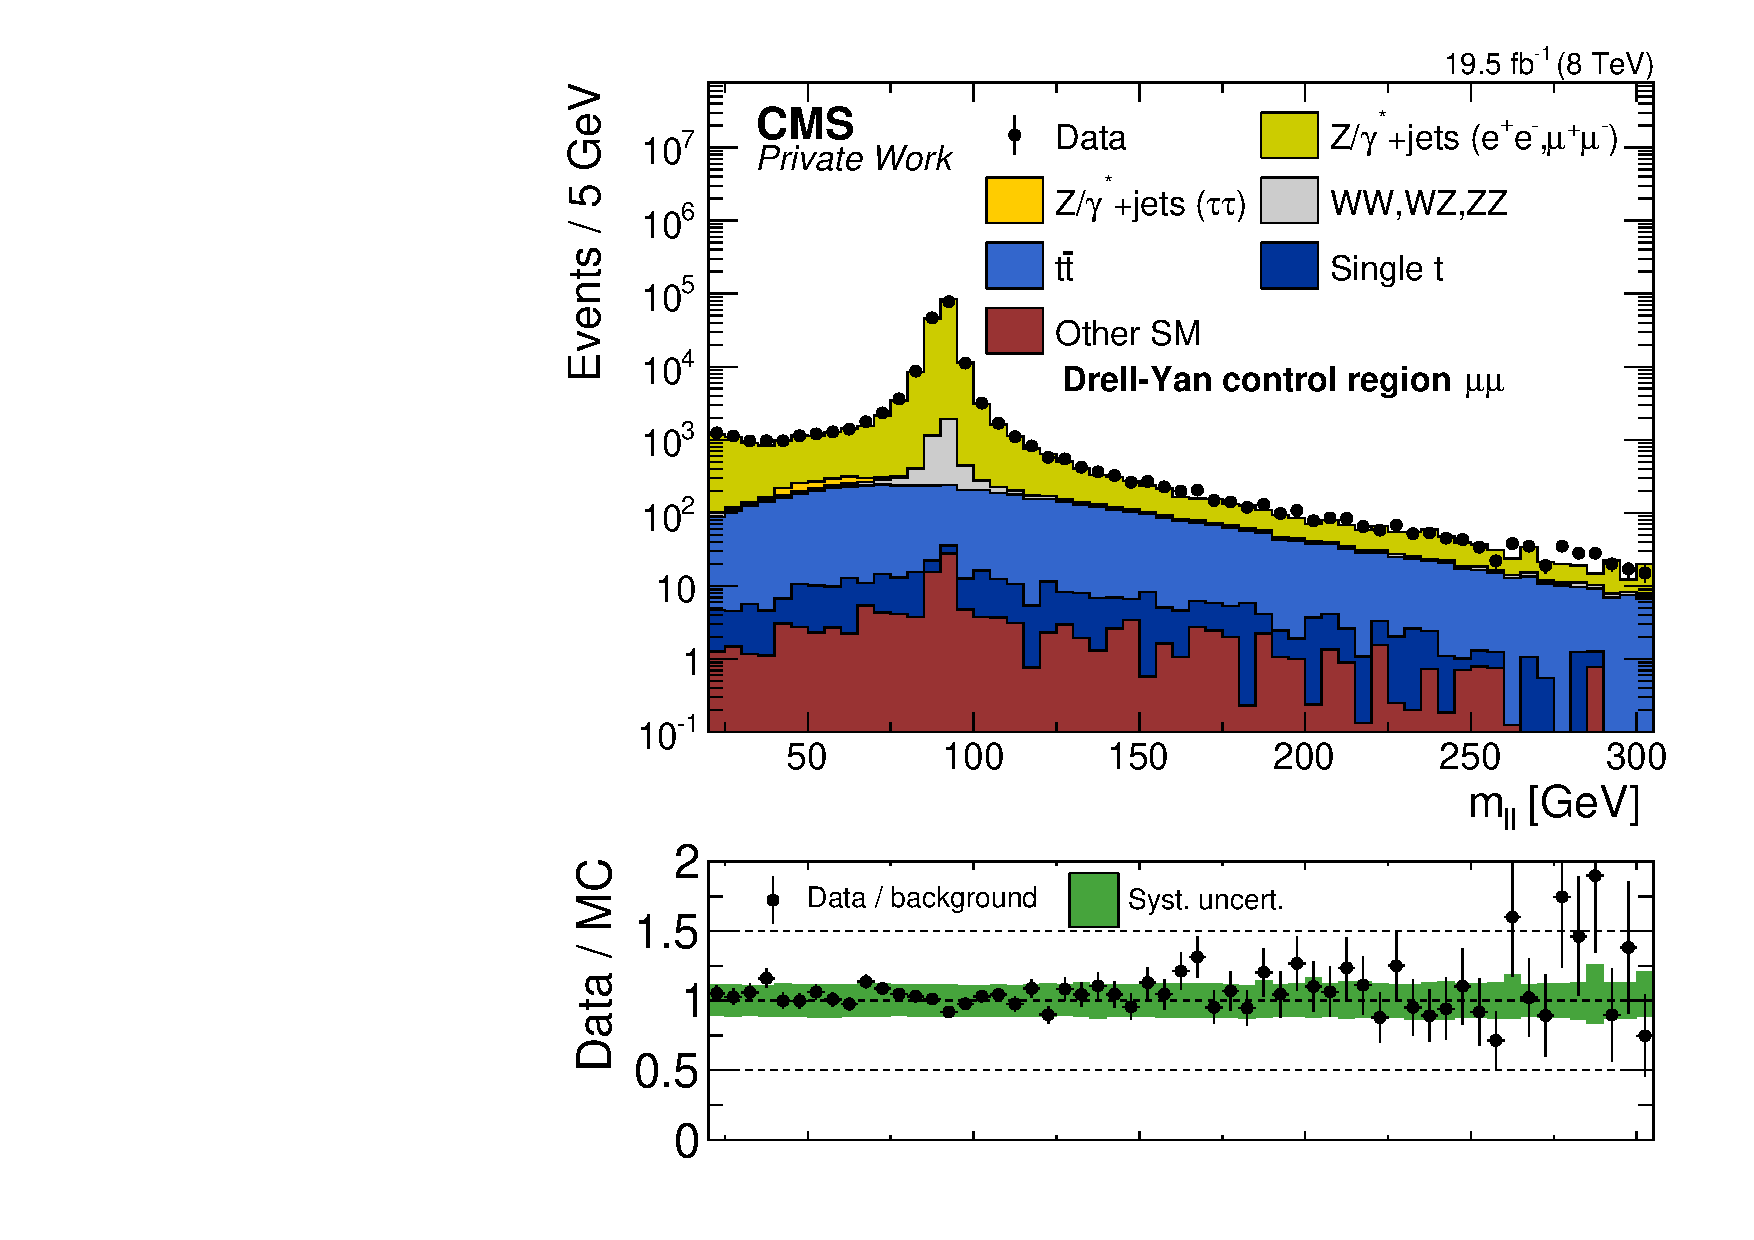
\includegraphics[width=\textwidth]{plots/BG/rmue/DrellYanControl_Mll_Full2012_MuMu_TopReweighted.pdf}
\end{minipage}
\begin{minipage}[t]{0.49\textwidth}
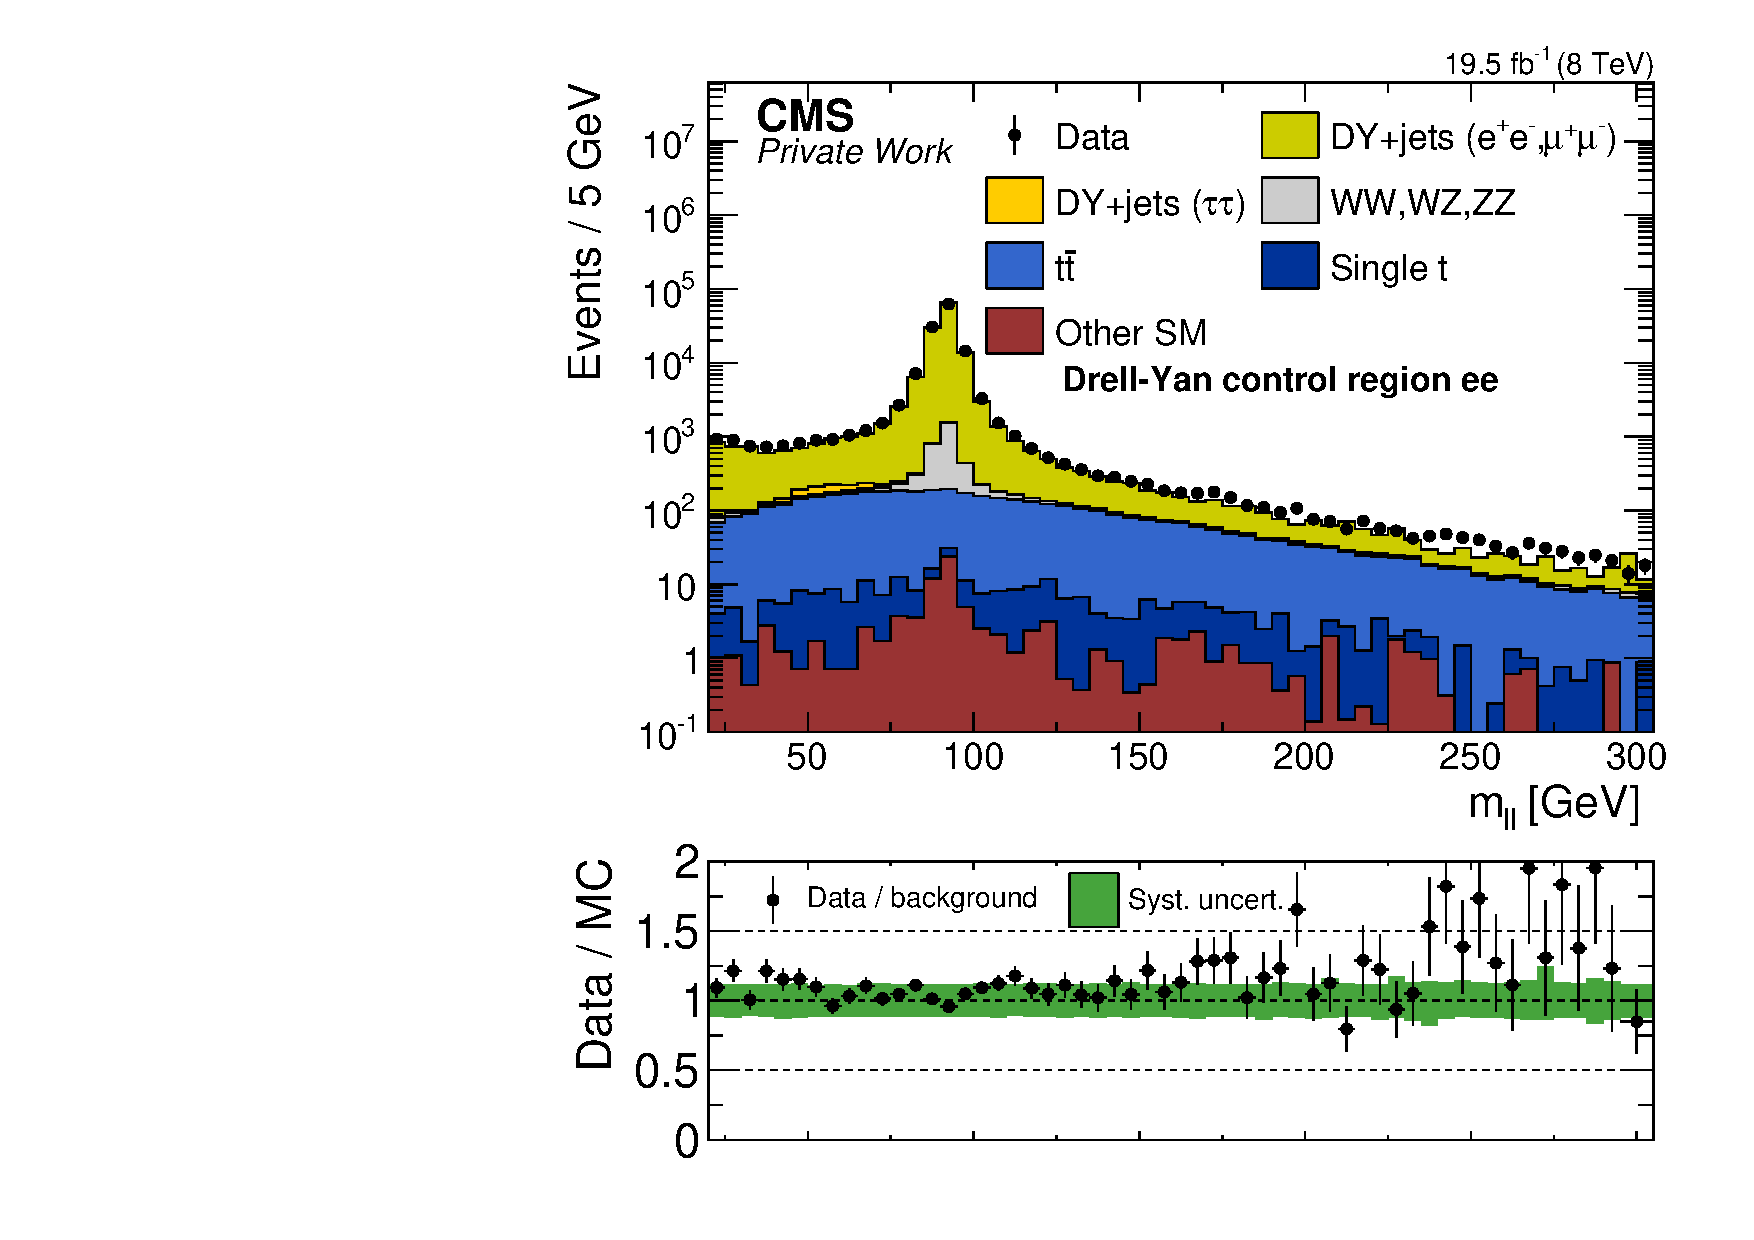
\includegraphics[width=\textwidth]{plots/BG/rmue/DrellYanControl_Mll_Full2012_EE_TopReweighted.pdf}
\end{minipage}
\caption{Distribution of \mll in the Drell-Yan control region for \MM events (left) and \EE events (right). The data is shown as the black dots, while the contributions from Standard Model processes, estimated from simulation, are shown as the stacked histograms.}
\label{fig:rmueMll}
\end{figure} 
The results of the calculation of \rmue are shown in Table~\ref{tab:RValuesControl}. Given are the observed yields for \MM and \EE events and the resulting value of \rmue with statistical and systematic uncertainties. In the central lepton selection, the \MM yield is about 18\% higher than the \EE yield. Similar results are observed on Drell-Yan simulation. For events with leptons in the forward region, a larger asymmetry between muons and electrons is observed, here the \MM yield is about 40\% higher than the \EE yield. 
\begin{table}[hbp]  \centering \renewcommand{\arraystretch}{1.2} \begin{tabular}{l|c|c|c}     
     & $n_{\mu\mu}$ & $n_{ee}$ & $r_{\mu e} \pm \sigma_{stat} \pm \sigma_{syst}$    \\    \hline
\multicolumn{4}{c}{Central} \\ \hline
    $MC$ & $              96205$ & $              79148$ & $              1.103\pm               0.004^{+              0.117}_{-              0.117}$    \\ 
    $Data$ & $              99144$ & $              83761$ & $              1.088\pm               0.003^{+              0.109}_{-              0.109}$    \\    \hline   
\multicolumn{4}{c}{Forward} \\ \hline    
    $MC$ & $              65017$ & $              44504$ & $              1.209\pm               0.006^{+              0.246}_{-              0.246}$    \\ 
    $Data$ & $              62778$ & $              44829$ & $              1.183\pm               0.004^{+              0.237}_{-              0.237}$    \\    \hline     
\end{tabular}  
\caption{$r_{\mu e}$ values for data and MC determined in the Drell-Yan control region, separately for the central and forward lepton selection.} 
\label{tab:RValuesControl}
\end{table}
The systematic uncertainties of the measurement 10\% for the central and 20\% for the forward lepton selection. These values are obtained from studies of the dependency of \rmue on relevant observables. These are on the one hand properties of the lepton pairs, while on the other hand the jet multiplicity and \MET are studied to asses potential biases introduced when applying \Rsfof in the signal region. The dependencies of \rmue on \mll, \MET, and $N_{jets}$ are shown in Figure~\ref{fig:rmueDependencies}. Some dependency is observed in the case of \mll, where the values are higher for low \mll below the Z peak. This can be traced back to a dependency on the \pt of the leptons, where the efficiency for muons has a sharper turnon compared to electrons, for example for the dilepton triggers. In data, there is a strong effect visible around the Z peak for forward leptons. This is caused by a systematic shift of the position of the Z peak between electron and muons and is not a general property of \rmue, as is evident from the comparison with $t\bar{t}$ simulation shown in the upper right of Figure~\ref{fig:rmueDependencies}. No strong dependencies can be observed for \MET and $N_{jets}$ within the statistical uncertainties. All observed deviations from the central values are covered by the systematic uncertainties assigned to the measurement. Further information on the dependency studies can be found in Appendix~\ref{app:rmue}
\begin{figure}[htbp]
\centering
\begin{minipage}[t]{0.49\textwidth}
  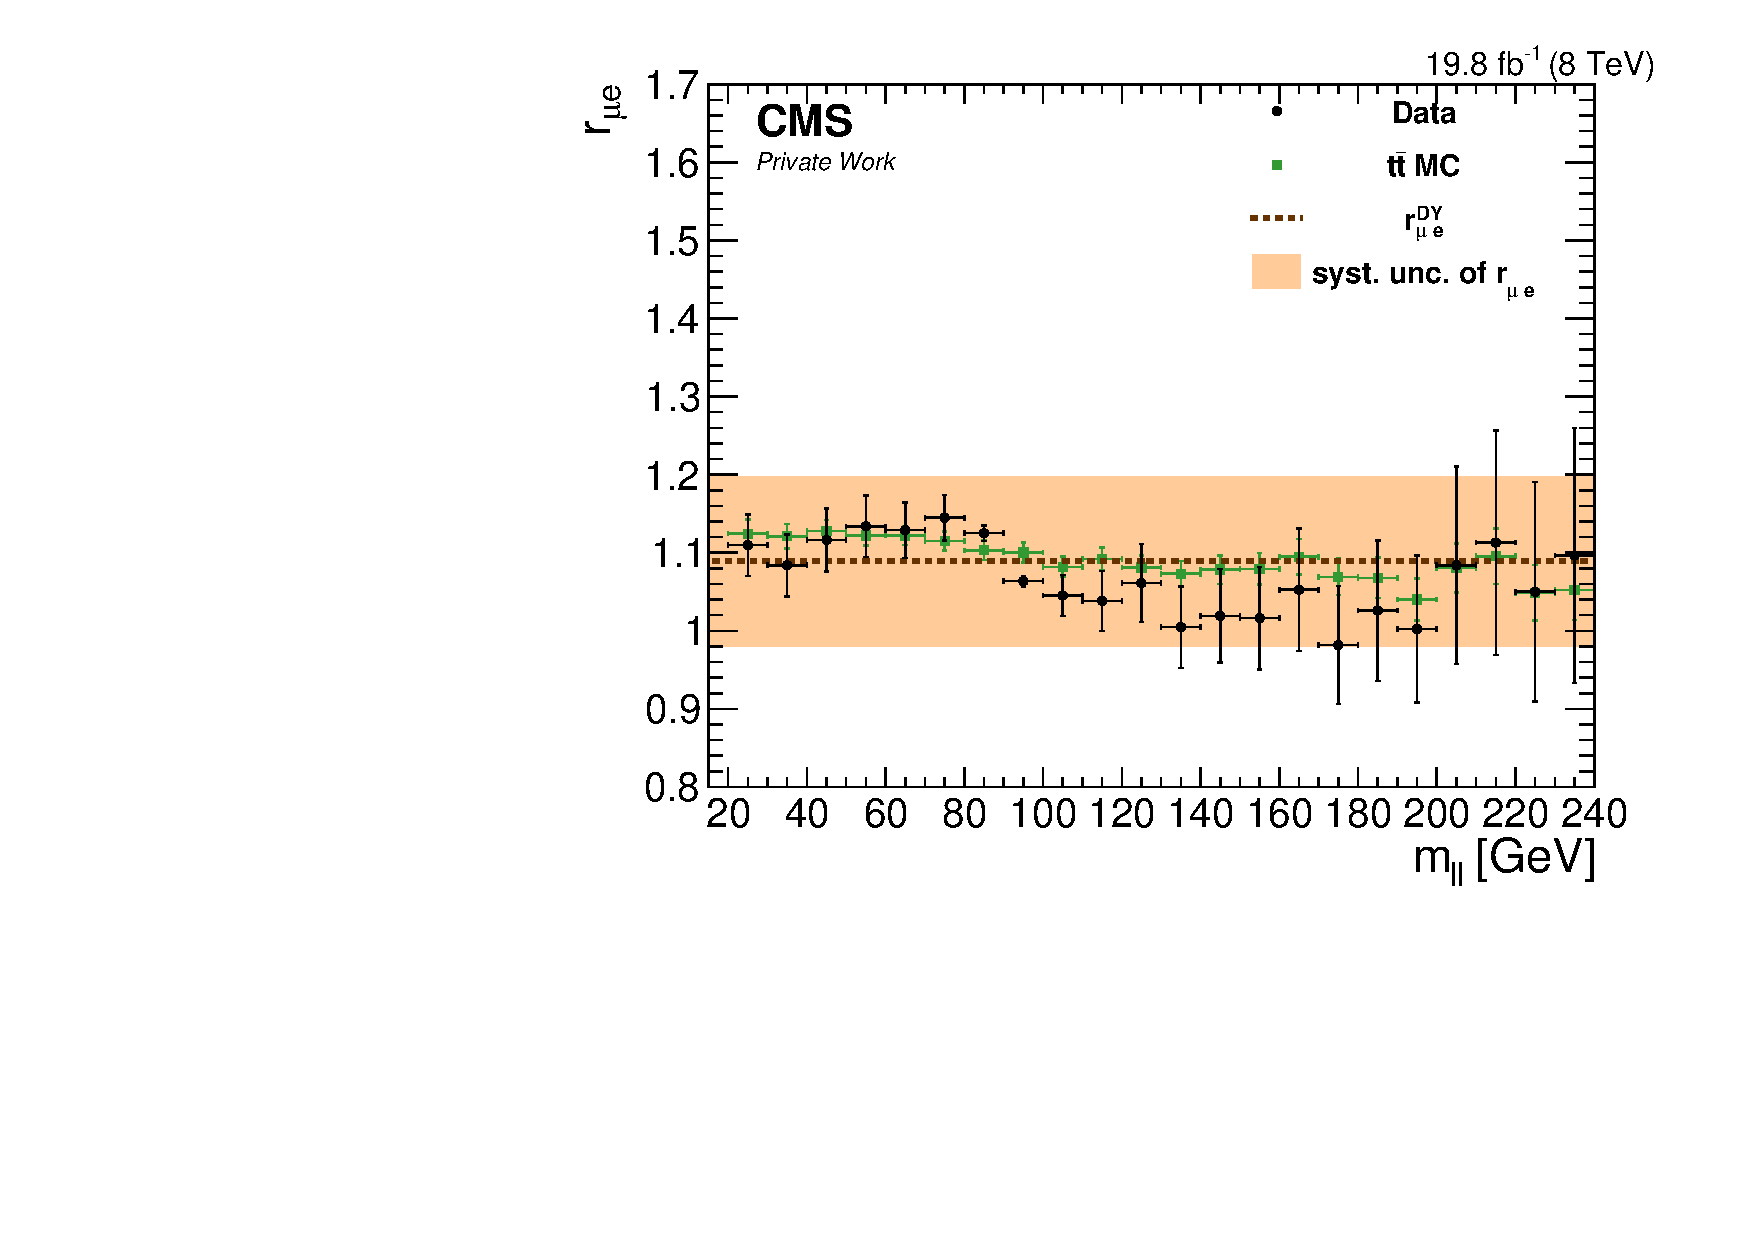
\includegraphics[width=\textwidth]{plots/BG/rmue/8TeVrRatioDataVsMCControl_mll_Central_Full2012.pdf}
\end{minipage}
\begin{minipage}[t]{0.49\textwidth}
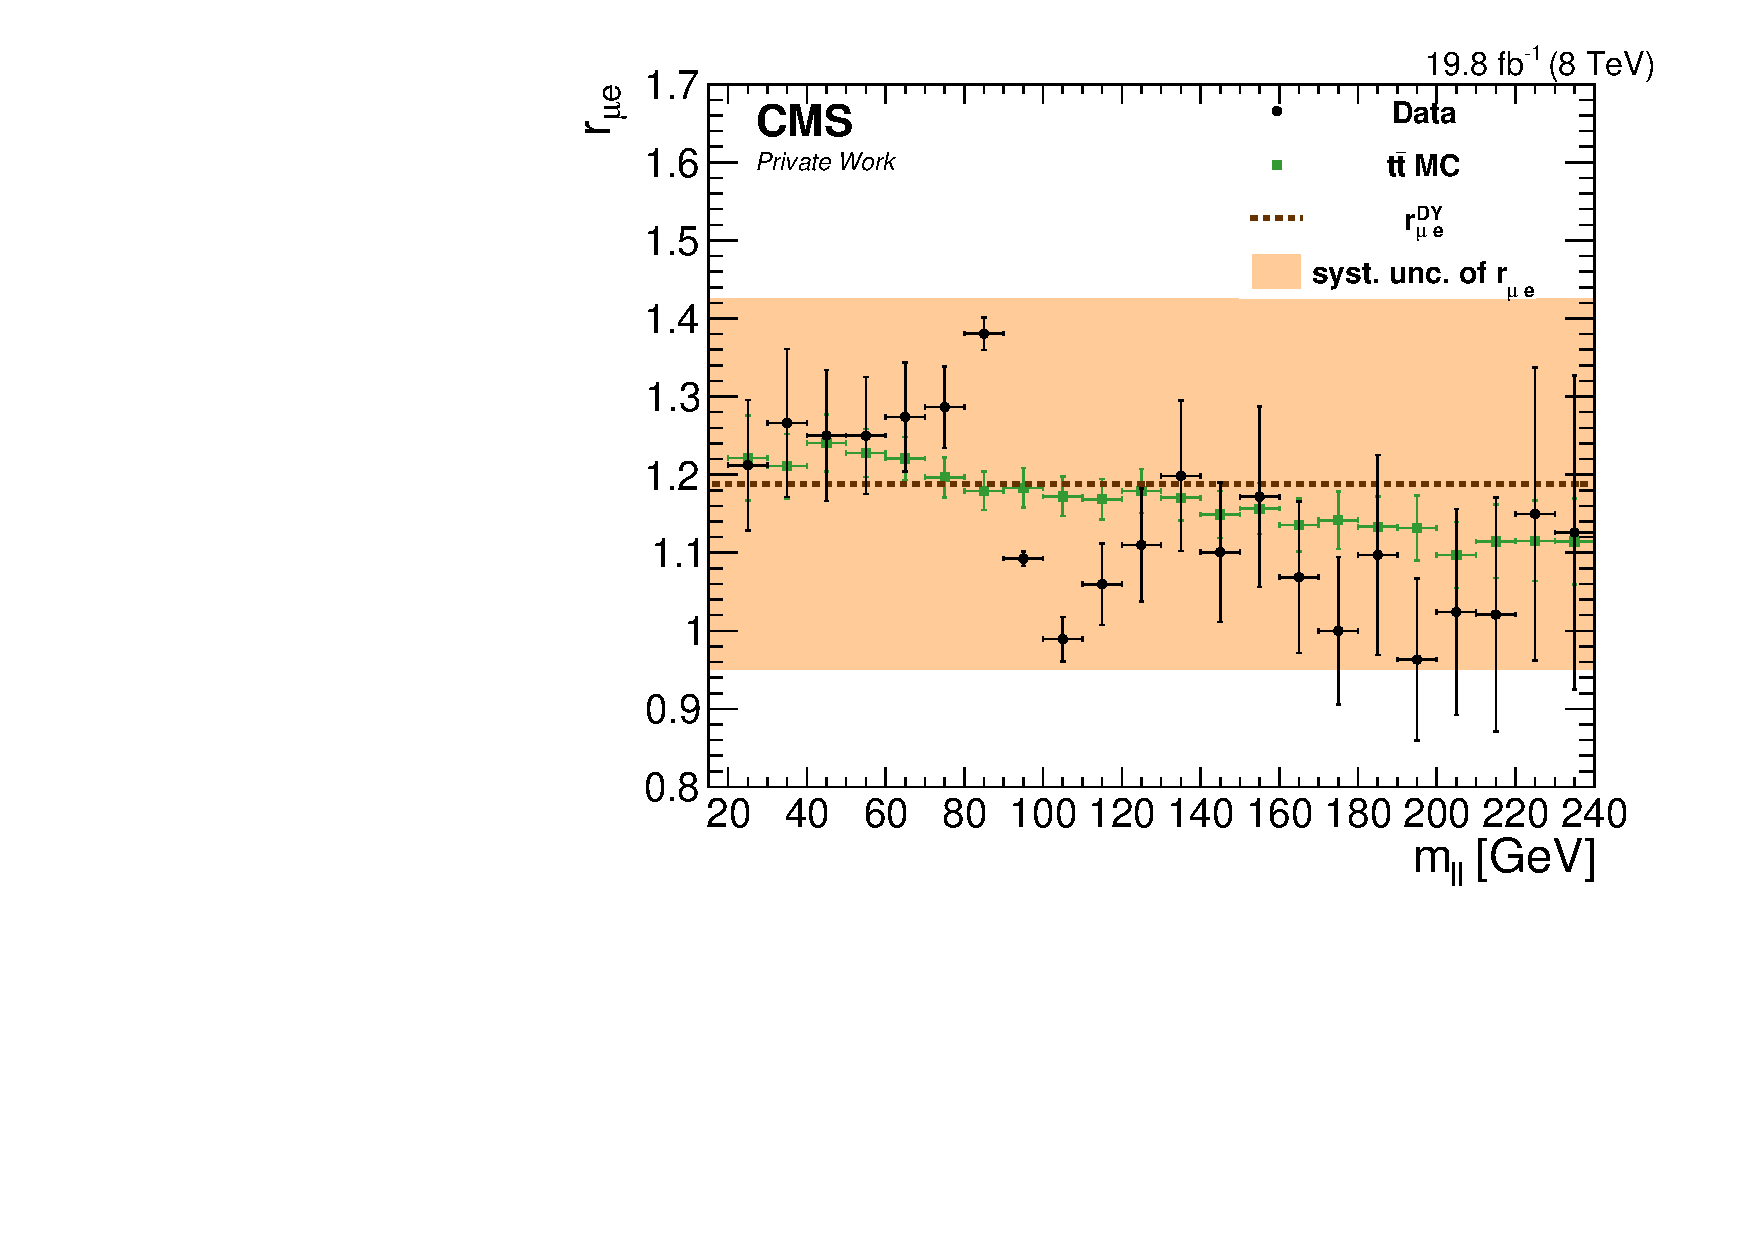
\includegraphics[width=\textwidth]{plots/BG/rmue/8TeVrRatioDataVsMCControl_mll_Forward_Full2012.pdf}
\end{minipage}
\begin{minipage}[t]{0.49\textwidth}
  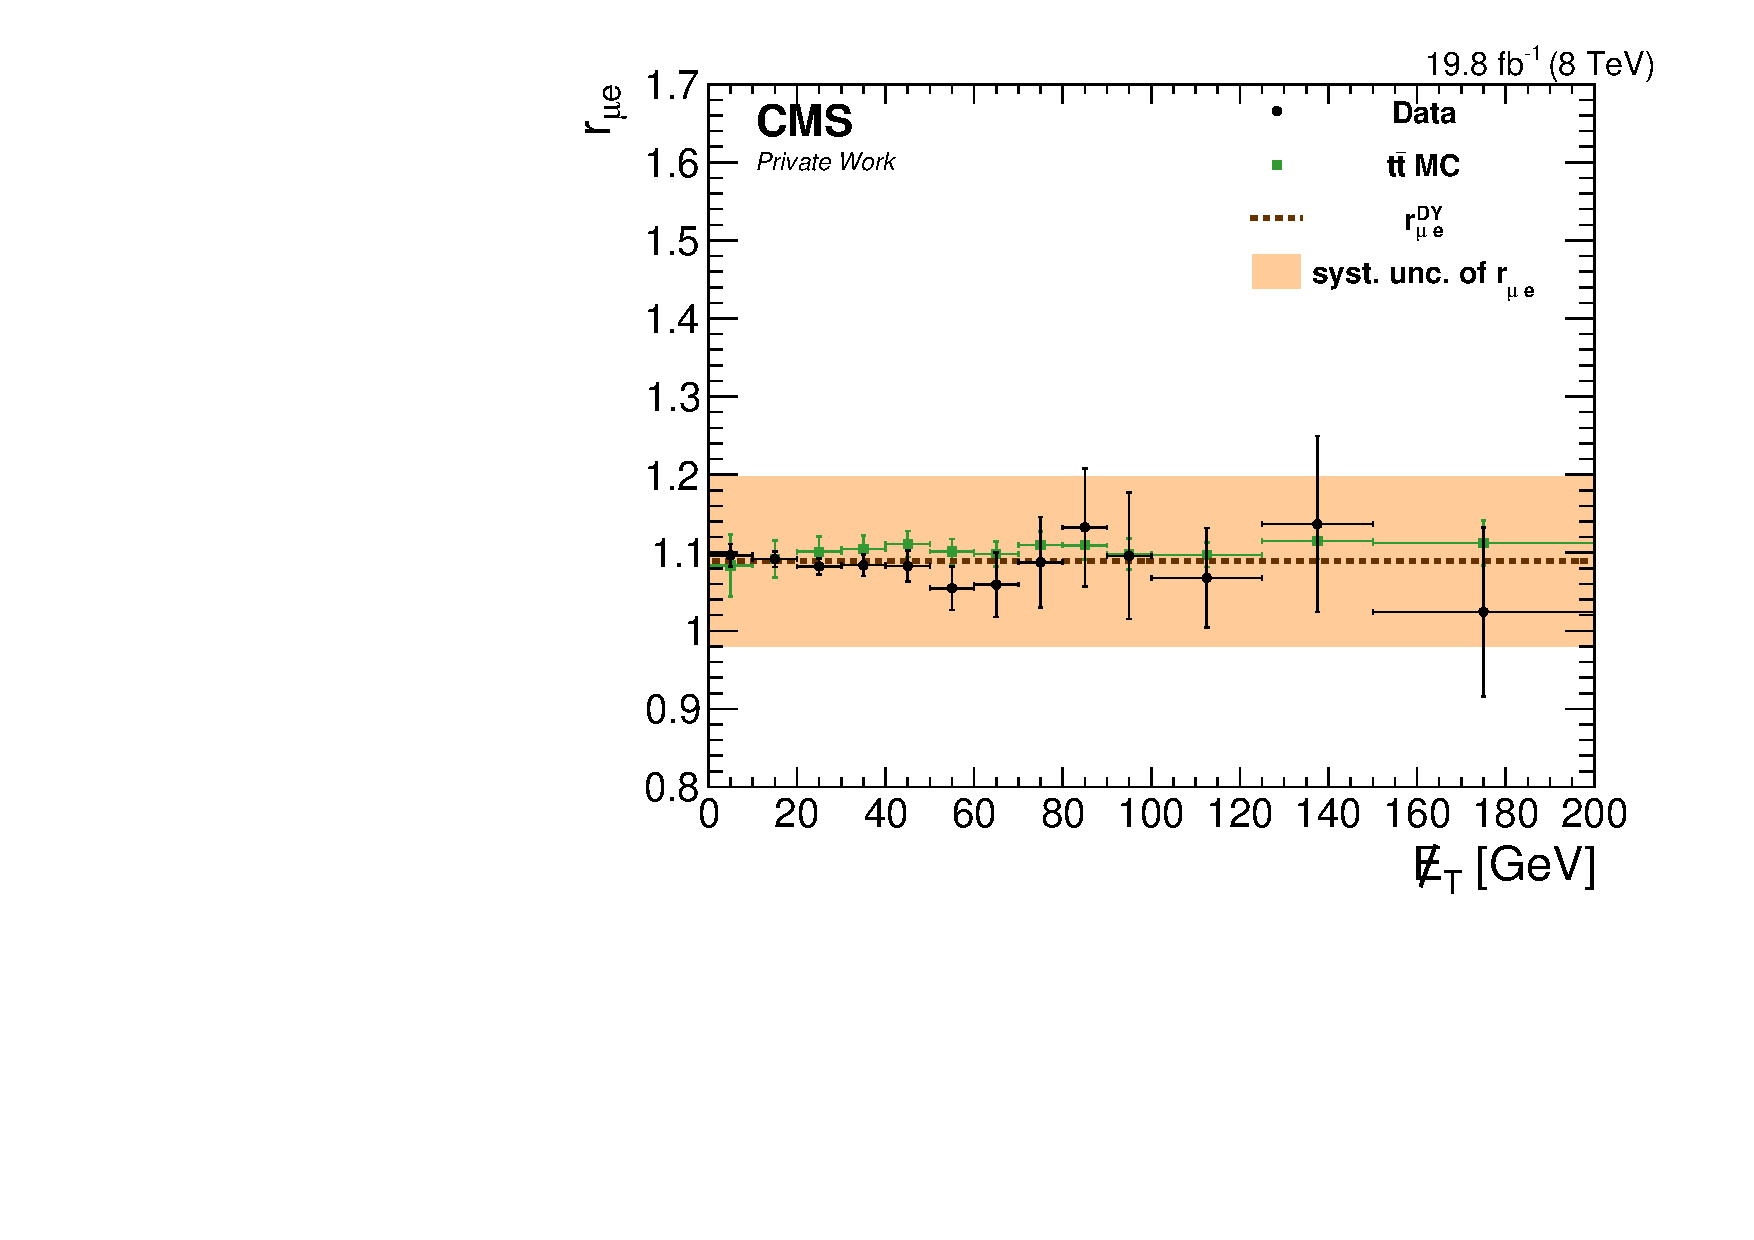
\includegraphics[width=\textwidth]{plots/BG/rmue/8TeVrRatioDataVsMCControl_met_Central_Full2012.pdf}
\end{minipage}
\begin{minipage}[t]{0.49\textwidth}
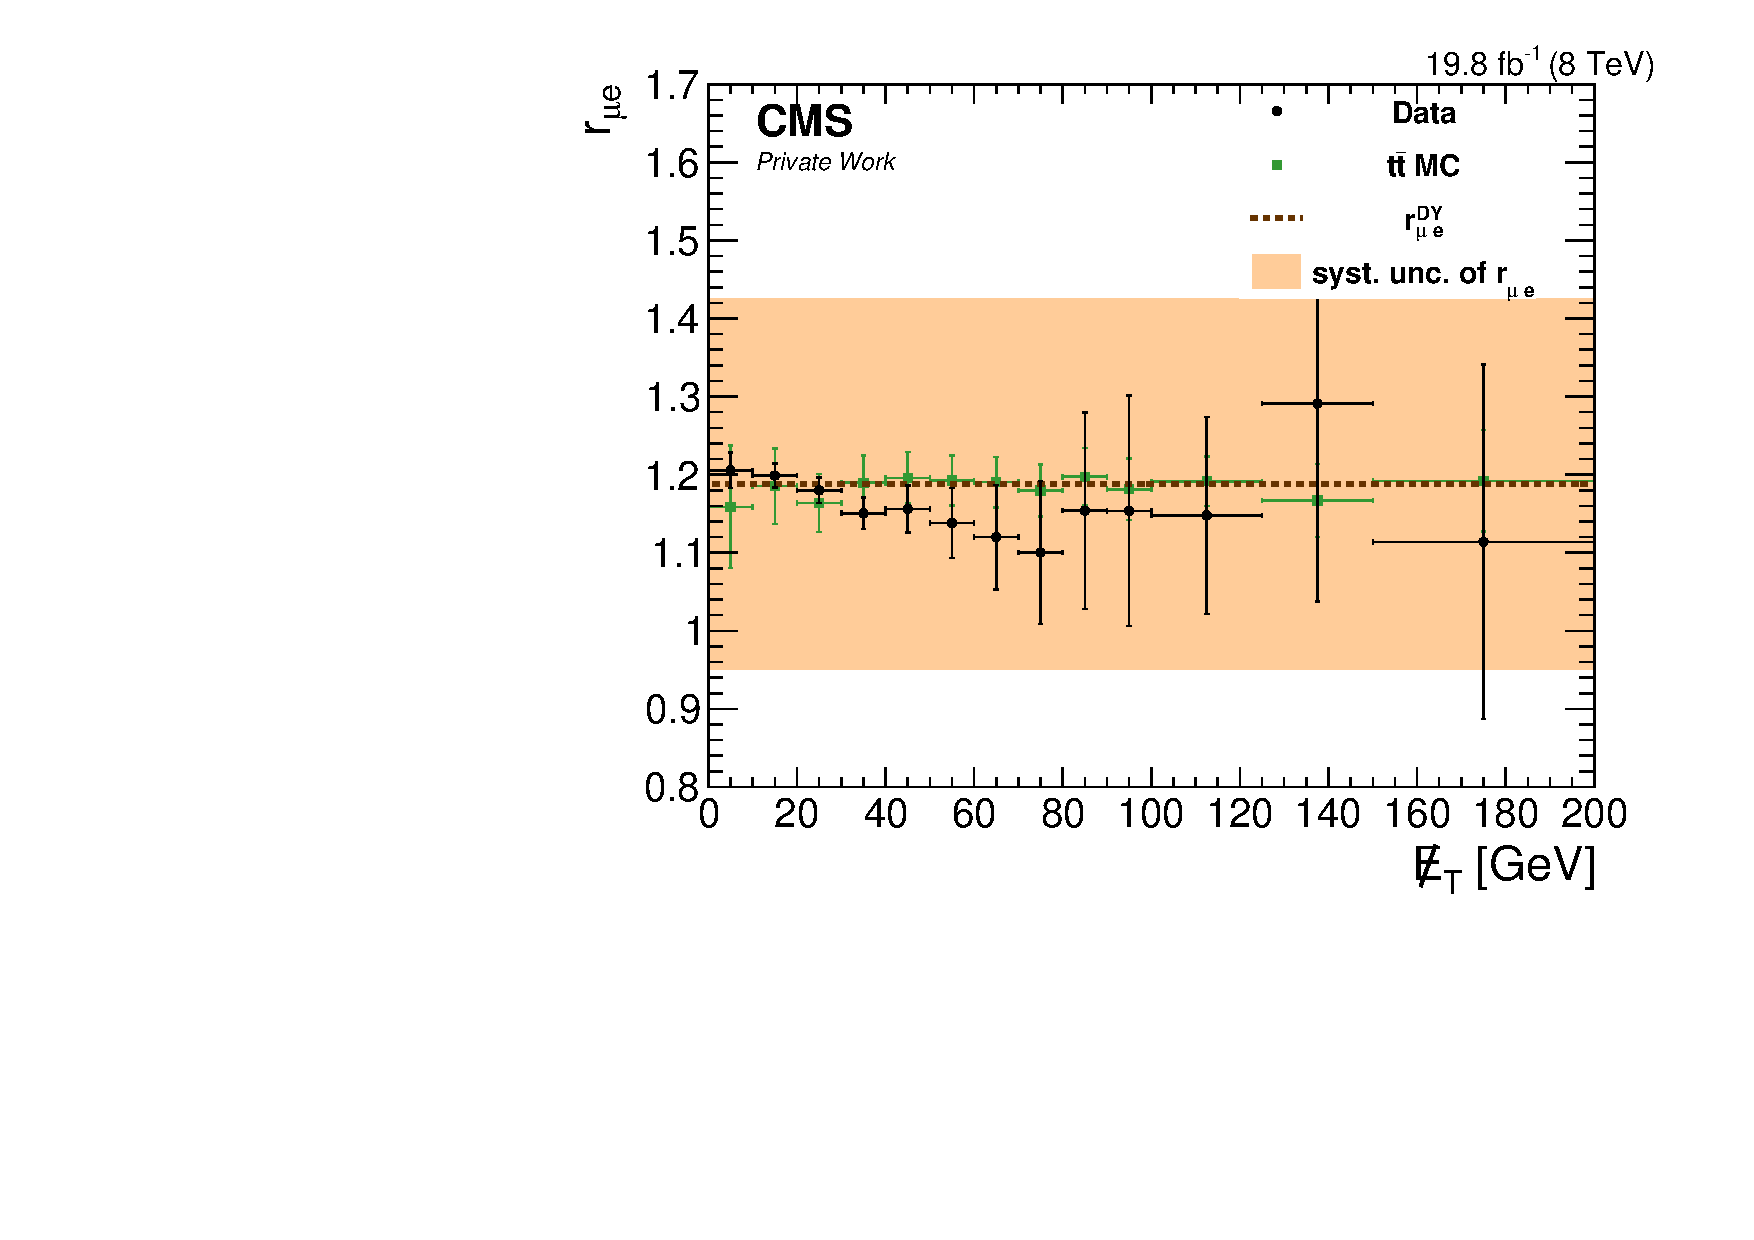
\includegraphics[width=\textwidth]{plots/BG/rmue/8TeVrRatioDataVsMCControl_met_Forward_Full2012.pdf}
\end{minipage}
\begin{minipage}[t]{0.49\textwidth}
  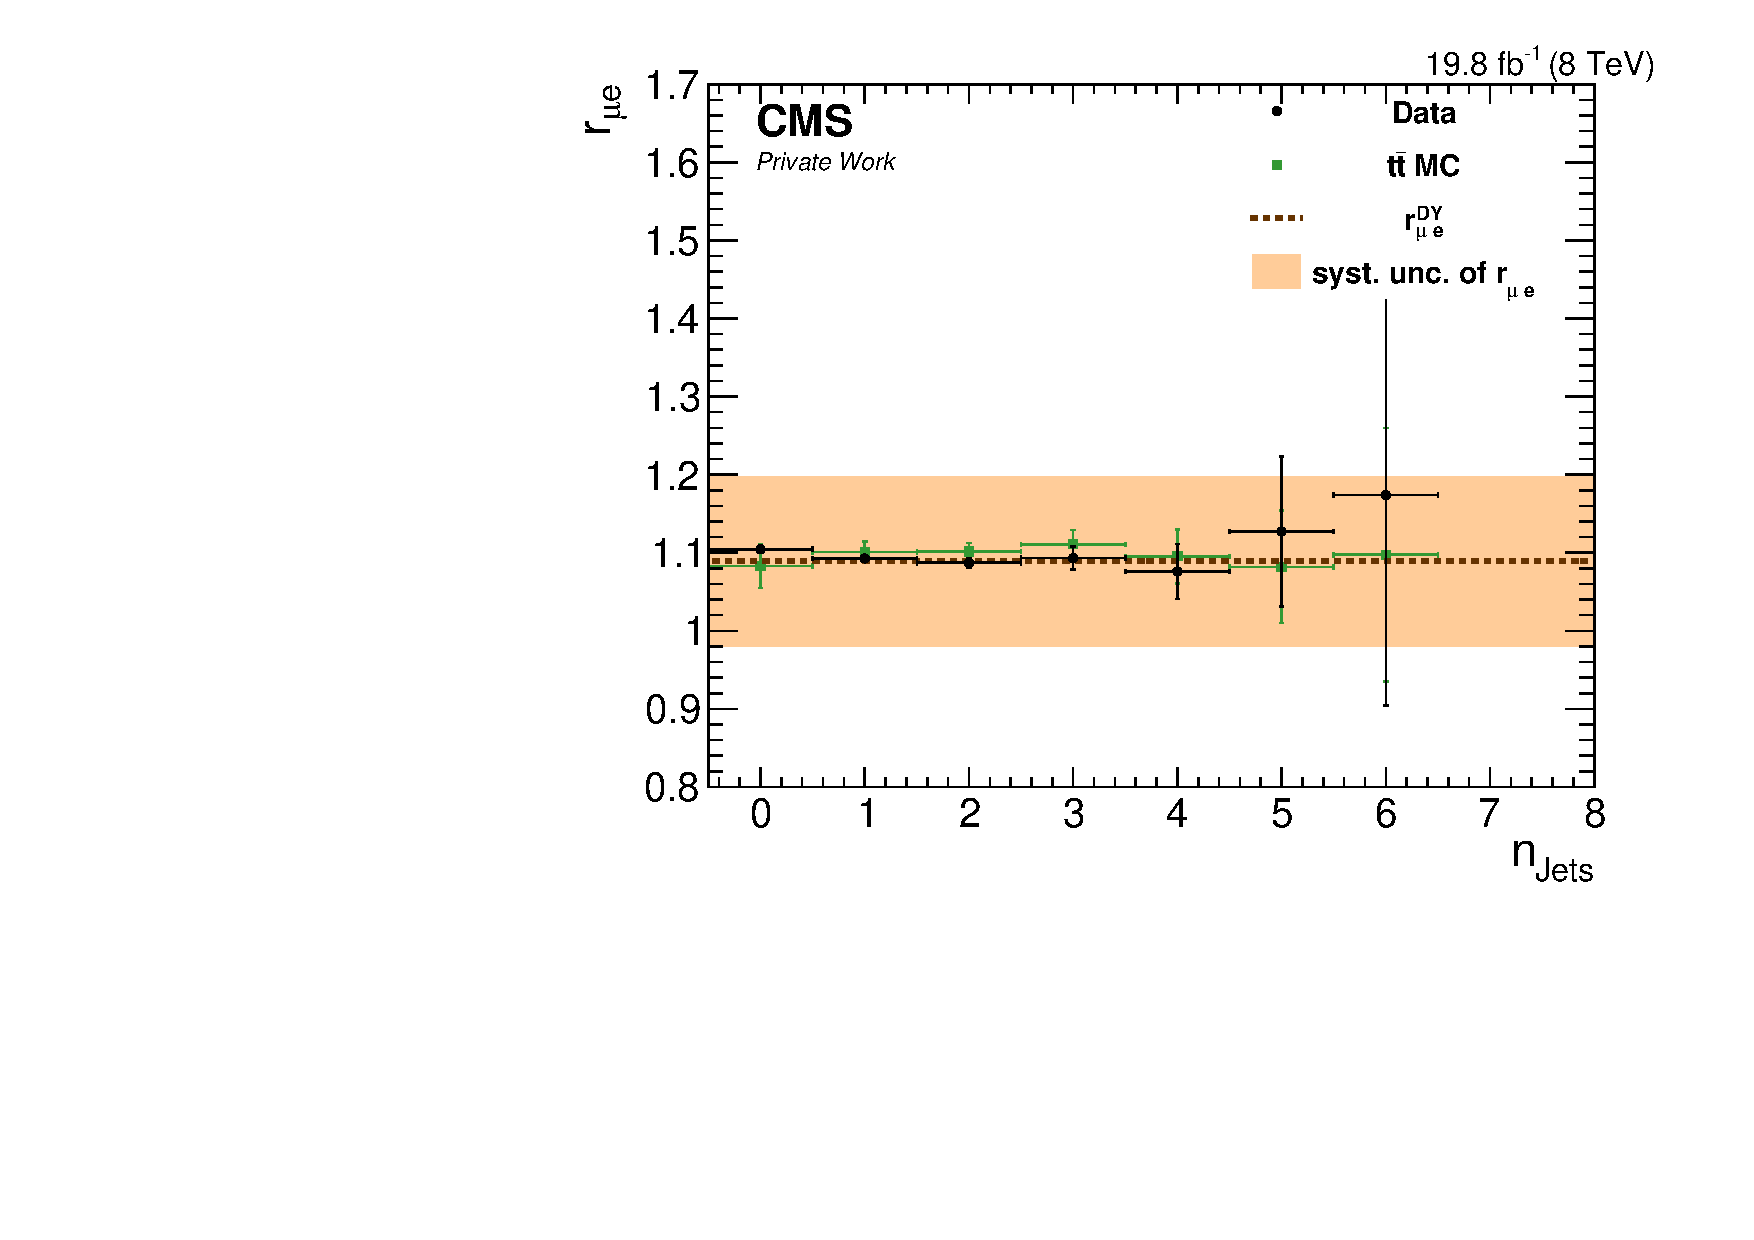
\includegraphics[width=\textwidth]{plots/BG/rmue/8TeVrRatioDataVsMCControl_nJets_Central_Full2012.pdf}
\end{minipage}
\begin{minipage}[t]{0.49\textwidth}
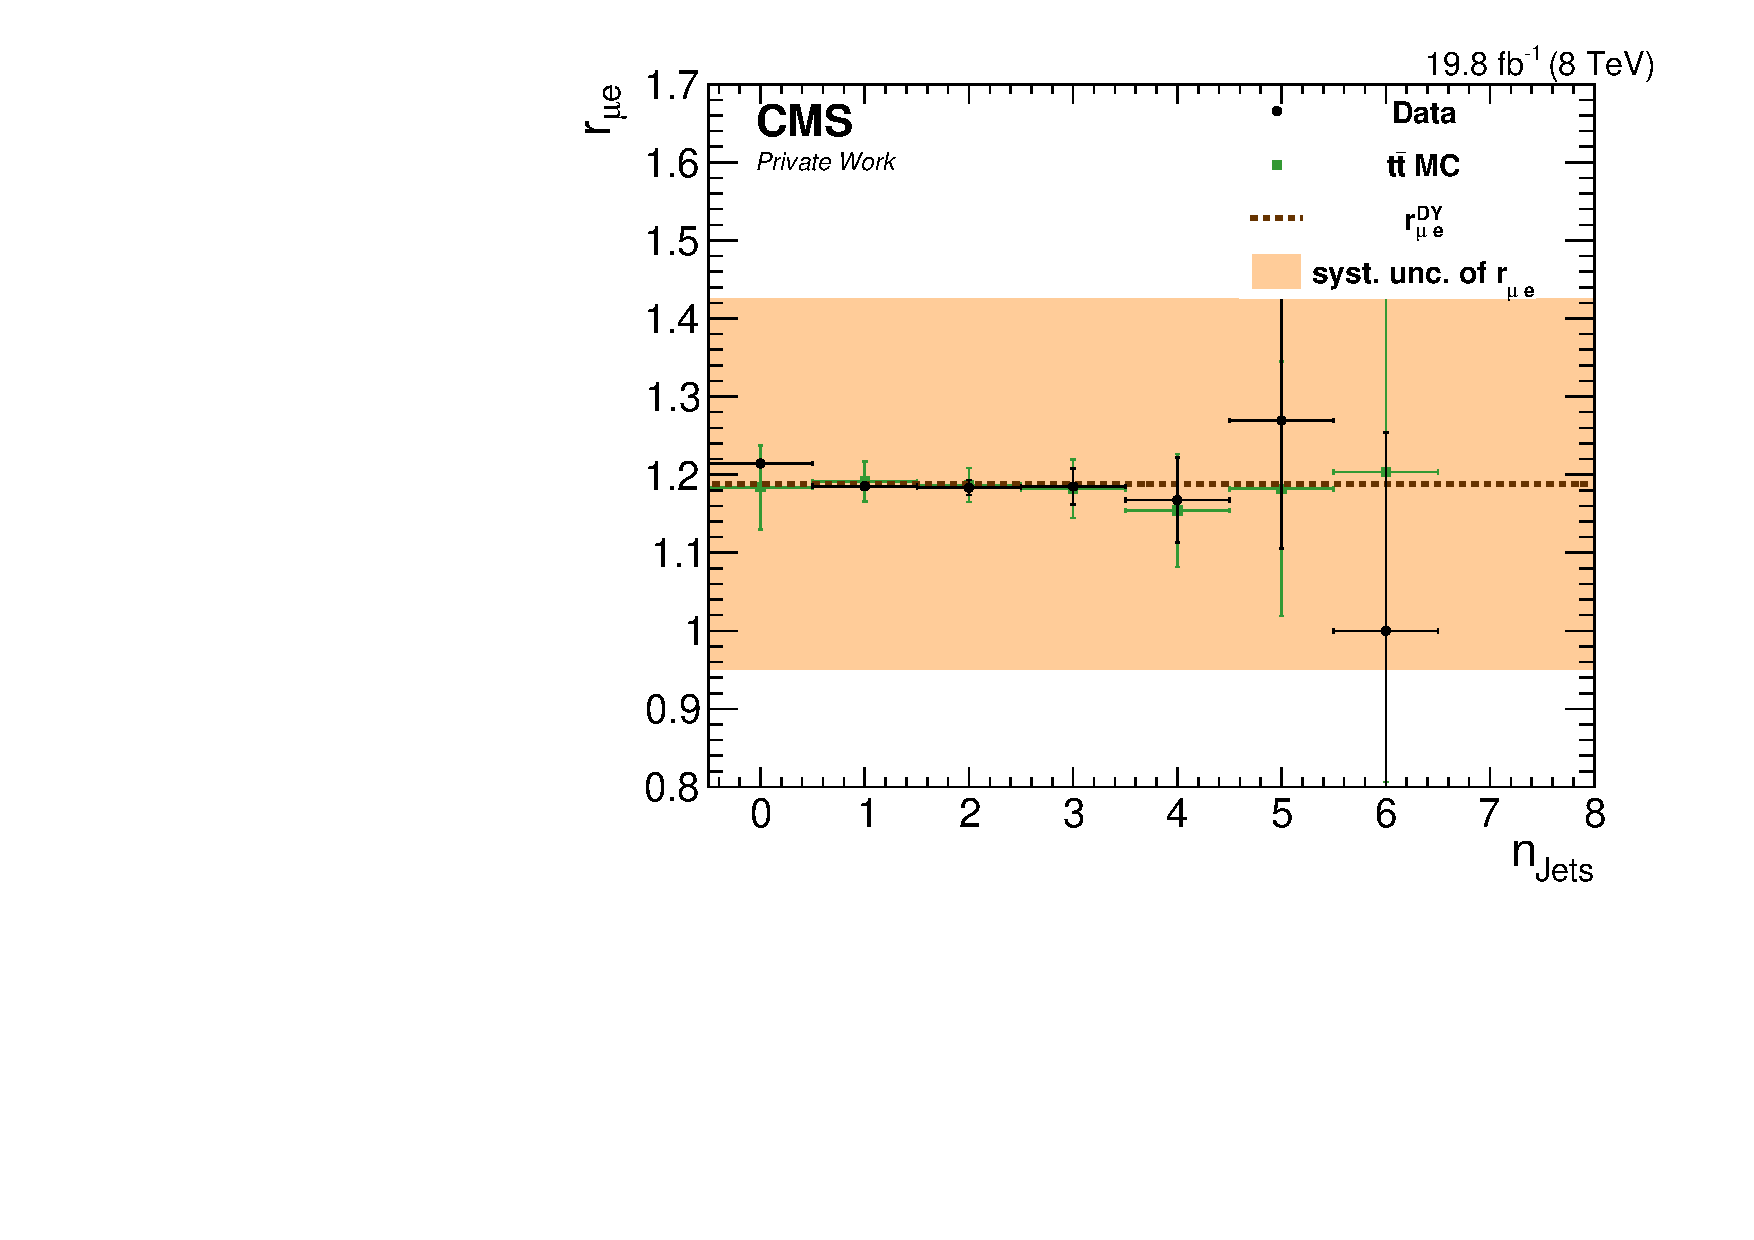
\includegraphics[width=\textwidth]{plots/BG/rmue/8TeVrRatioDataVsMCControl_nJets_Forward_Full2012.pdf}
\end{minipage}
\caption{Dependencies of \rmue on \mll (top), \MET (middle), and $N_{jets}$ (bottom) for the central (left) and forward (right) lepton selection. The results on data are shown in black while $t\bar{t}$ simulation is shown in green. The central value is shown as a brown dashed line while the systematic uncertainty is shown as an orange band.}
\label{fig:rmueDependencies}
\end{figure} 
\subsubsection{Measurement of \RT}

\section{Backgrounds containing a Z boson}
\section{Investigation of possible further backgrounds}
\section{Search for a kinematic edge with a fit}
